\chapter{Enviroment and Basics}
\label{cha:enviromentandbasics}

\section{Programming Tools}
As the target of this thesis is a mere proof of concept, the programming language of choice is matlab \cite{tool:matlab}. This is a reasonable decision because in the matlab language a huge part of the needed functionality concerning simple mathematical functions is already implemented and easy to use. \\
Pros:
\begin{itemize}
\item easy to use mathematical function.
\item fast and easy way to enter data.
\item good and simple ways of debugging and locating errors.
\end{itemize}
Cons:
\begin{itemize}
\item slow computation speed.
\item needs translation in other language ( e.g. c++ ) for further useage.
\end{itemize}

As versioning tool "git" \cite{tool:git} is used together with www.github.com as an open source storage platform for the resulting code.

\section{Basics}
For better understanding of the following chapters the central mathematical formulas are repeated here.
For the minkowski sum and convex hull \cite{minkowski} should give more information.
\subsection{Basic Vector Math} %representation with points
If the objects are represented as a list of corner points, vector math comes in handy when describing the borders of the object.
Let A be a simple object defined by the following list:
\begin{align*}
A = 	&( 0 , 0 ;2 , 0 ;2, 2; 0, 2)	
\end{align*}

Each pair x,y defines one corner of A and the points are ordered to travel along the border of A counterclockwise.
The lines connecting these points will be called the borders of A. They are calculated by substracting the points from each other such that the vectors point along the border clockwise. This leads to:
\begin{align*}
A_{vec} = 	&( 2 , 0 ; 0 ,2 ;-2, 0; 0, -2)	
\end{align*}

\begin{figure}[H]
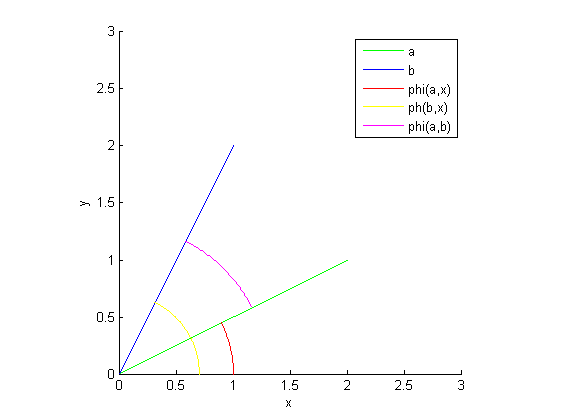
\includegraphics{VectorDegree}
\caption{Figure showing the calculation of the angle difference between vectors $a$ and $b$ via reference to x-axis}
 \end{figure}

Next will be the calculation of the angle beetween two lines $a$ and $b$. This is done by taking a reference vector, for example the x-axis r=$(1,0)$. Calculating the angle to that and building the difference in angle results in the relativ anlge difference beetween $a$ and $b$. This angle tells us which vector lies "below" the other by looking wether its signed or not.\\
The formula for this is:
\begin{align*}
  \phi_{a,b} &= \phi_{a,r} - \phi_{b,r}\\
	&= tan^{-1} ( \frac{ a(2) }{  a(1) } ) - tan^{-1} ( \frac{b(2)}{b(1)}); 
\end{align*}
Another vector is necessary as a reference to determine if the difference of the vectors angles is positiv or negativ. This information is needed to build the convex hull.


\subsection{Minkowski Sum}
The minkowski sum is needed to calculate the convex hull beetween two polyhedra $A$ and $B$. The formula for the Minkowski sum is as follows:
\begin{align*}
 A + B = \{\mathbf{a}+\mathbf{b}\,|\,\mathbf{a}\in A,\ \mathbf{b}\in B\}. 
\end{align*}
$A$ and $B$ are a set of points in 2 dimensional space defining a convex polyhedron. 

\subsection{Convex Hull} %collision representation with points
Furthermore we define the center of these objects to be $M_A = (1,1)$ and $M_B = (0.5 , 1)$.
The convex hull for A to B is calculated with the minkowski sum of A' and B' with
\begin{align*}
A'  &= \{ -(\mathbf{a} - M_A) |\mathbf{a} \in A \}\\
B'  &= \{ \mathbf{b} - M_B |\mathbf{b} \in B \}\\
\end{align*}
Basically this means that the points of A are shifted with $-M_A$ and mirrored at $M_A$ before being added to each point of B shifted with $-M_B$ and then reshifted with $M_A$ to get a list $C_{temp}$ of $4\cdot 4 = 16$  points.
\begin{align*}
A &= 	( 0 , 0; 2 , 0; 2, 2; 0, 2), M_A =( 1, 1)\\
B &= (0, 0; 1, 0; 1, 1; 0, 1),  M_B =(0.5, 0.5)\\
A' &= (1, 1; -1, 1; -1, -1; 1, -1)\\
B' &= (-0.5, -0.5; 0.5, -0.5; 0.5, 0.5; -0.5; 0.5)\\
C_{temp} &=	\begin{matrix}
		(&0.5, &0.5; &1.5, &0.5; &1.5, &1.5; &0.5, &1.5;\\
		&-1.5, &0.5; &-0.5, &0.5; &-0.5, &1.5; &-1.5, &1.5;\\
		&-1.5, &-1.5; &-0.5, &-1.5; &-0.5, &-0.5; &-1.5, &-0.5;\\
		&0.5, &-1.5; &1.5, &-1.5; &1.5, &-0.5; &0.5, &-0.5)
		\end{matrix}\\
C_{temp_shifted} &= \begin{matrix}
		(&1.5, &1.5; &2.5, &1.5; &2.5, &2.5; &1.5, &2.5;\\
		&-0.5, &1.5; &0.5, &1.5; &0.5, &2.5; &0.5, &2.5;\\
		&-0.5, &-0.5; &0.5, &-0.5; &0.5, &0.5; &-0.5, &0.5;\\
		&1.5, &-0.5; &2.5, &-0.5; &2.5, &0.5; &1.5, &0.5)
		\end{matrix}\\
\end{align*}
Each line represents one point of A with the points of B added. By choosing the outer points from $C_{temp}$ and put them in $C$, such that no point from $C_{temp}$ is still outside $C$  we will get an object C which defines the space around B which the object A can not enter or they will collide. The points can be choosen by searching for the combinations of minimum/maximum $x$ and $y$ coordinates in C.
\begin{align*}
C = (-0.5, -0.5; 2.5, -0.5; 2.5, 2.5; -0.5, 2.5)
\end{align*}

\subsection{Pathfinding Algorithms on Graphs}
Pathfinding in general describes the way of finding a path beetween two points in a graph or net of nodes. The two major algorithms currently in use are A$^\star$ and Dijkstra's algorithm. As A$^\star$ is a variant of Dijkstra's algorithm, Dijkstra's will be explained first and afterwards the differences will be highlighted.\\
Dijkstra's algorithm uses a weighted graph and begins on a starting node which is connected to a set of adjacent nodes. These adjacent nodes are the starting rim.
Dijkstra works in these steps:
\begin{enumerate}
\item Take unvisited node with shortest distance to the start from rim and check if it is the target node.
\item If not target node, try to add all adjacent nodes to rim.
\begin{itemize}
\item If adjacent node is not in rim, insert the node with its predecessor and distance.
\item If adjacent node is in rim check distance:
\begin{itemize}
\item If adjacent nodes distance is higher than node in rim, discard said node.
\item If adjacent nodes distance is smaller than node in rim, update predecessor and distance.
\end{itemize}
\end{itemize}
\item Mark node as visited and repeat.
\end{enumerate} 
As long as it is guaranteed that no negativ distance occurs in the search graph, Dijkstra is bound to return the shortest possible path.\\\\
A$^\star$ is a variant which adds a heuristic function measuring the distance beetween the current node and the target. The heuristic and the distance to the start build a weighted sum. This results in a faster exclusion of possibly wrong paths, but it no longer guarantees to find the optimal path.